\subsection{Pipeline View}

\begin{figure}[htbp]
\centering
\vspace{-2mm}
 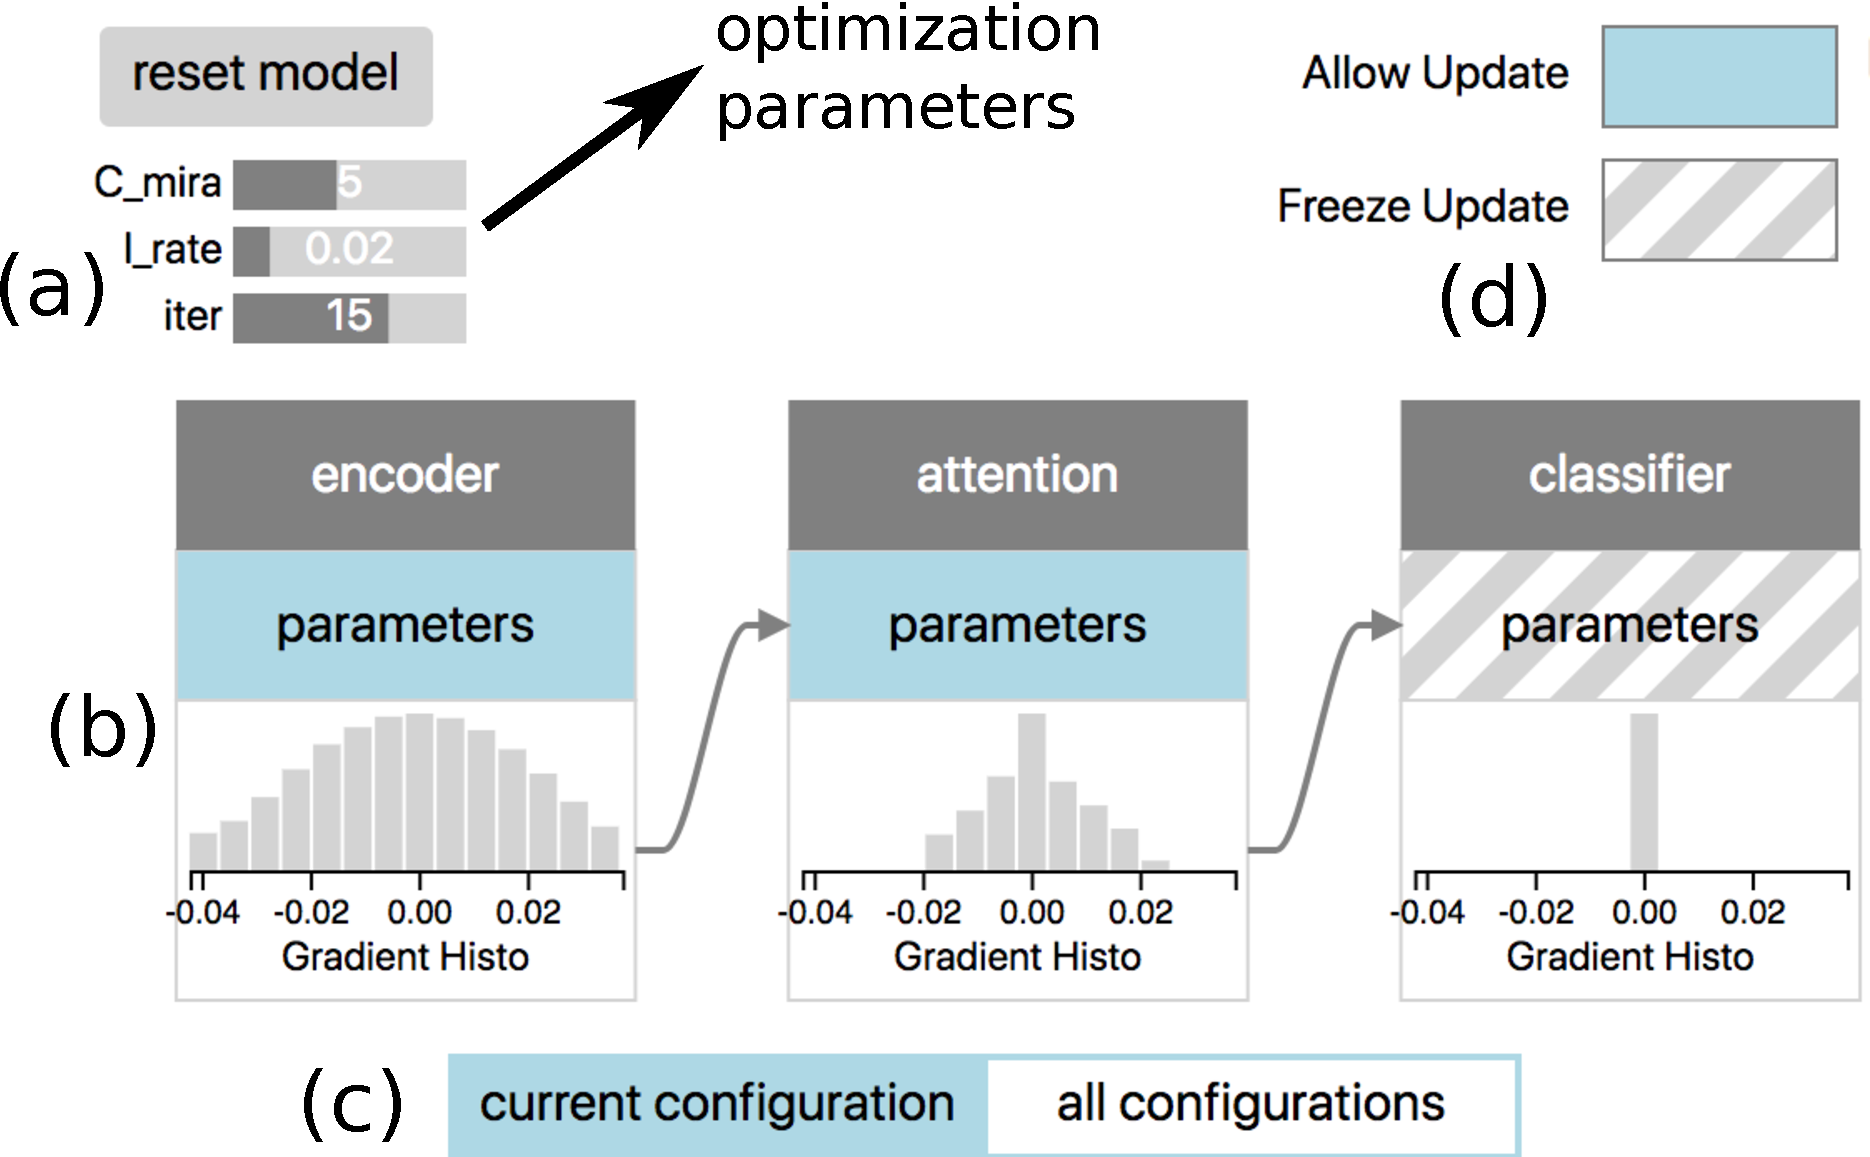
\includegraphics[width=1.0\linewidth]{pipelineView}
 \caption{
Visual representation of the three stages (encoder, attention, classifier) model. In the proposed tool, we allow the model parameter to be updated to fix a prediction error. The pipeline view, by showing the aggregated gradient distribution, inform the user about the how different part of the model response to the optimization.
%
The optimization parameters is shown in (a), each of the stages is illustrated in (b), where the user can click on the parameter bar to enable or disable its update (the legend about its state is shown in (d) ). In (c), we select whether if we want to use current update setting as display or try all the configuration combination (i.e., update for each stage can be enabled or disabled).
 }
\label{fig:modelPipeline}
\end{figure}

\subsubsection{Margin-Infused Relaxed Algorithm (MIRA)}
the mira loss is $|w' - w|^2 + C * J(w')$
